\section{Arkitektur}
Den overordnede arkitekturskissen, figur \ref{fig:overordnet-ark}, 
beskriver den overordnede helheten i systemet. En sensor plasseres på 
hjul/nav på lastebilen. Denne sender vibrasjonsfrekvenssignaler til en 
prosesseringsenhet plassert sentralt i lastebilen. I prosesseringsenheten 
tolkes frekvenssignalet, og dersom det detekteres en anomalitet i 
frekvensområdet, rapporteres dette i et lesbart format opp til en 
smartskjerm montert i dashbordet i førerhuset på lastebilen.
\newline
\begin{figure}[H]
	\centering
	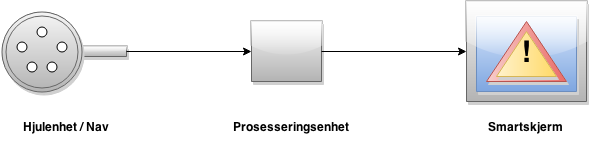
\includegraphics[width=1.00\textwidth]{images/arkitektur-overordnet.png}
	\label{fig:overordnet-ark}
	\caption{Overordnet arkitekturskisse.}
\end{figure}

\subsection{Model-view-controller}
\label{sec:arkitektur}
Presentasjon av varsling opp til førerhus, implementeres som MVC-pattern, 
hvor den sentrale prosesseringsenheten har controller-rollen og gjør alle 
de sentrale utregningene for systemet. Controlleren sender de prosesserte 
dataene til viewet, som i denne sammenhengen er smartskjermen plassert i 
dashbordet. Ved utvidelse til støtte for rapportering av spesifikke, 
kjente feil, implementeres modelstøtte i prosesseringsenheten som en 
``database'' av tupler bestående av signal og tilhørende feilmelding. 

Sammenhengen mellom modellen, viewet og controlleren ses i figur \ref{fig:mvc}.
\newline
\begin{figure}[H]
	\centering
	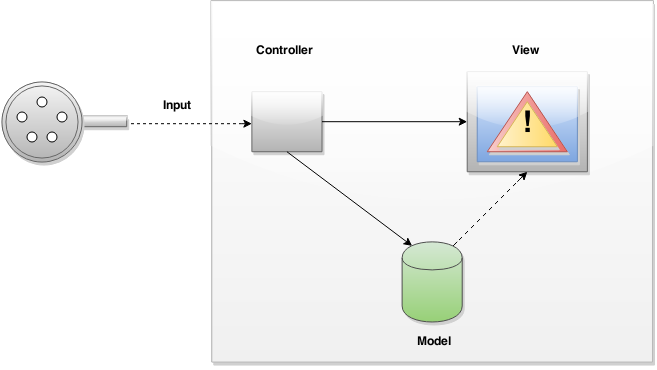
\includegraphics[width=1.00\textwidth]{images/architecture2-mvc.png}
	\label{fig:mvc}
	\caption{Arkitekturskisse: Model-view-controller.}
\end{figure}